\section{Der Gradient}
Der Gradient beschreibt einen Vektor, welcher in Richtung des steilsten Anstiegs einer Funktion zeigt.
Die Komponenten des Gradientenvektors bestehen aus den partiellen Ableitungen der Funktion an der jeweiligen Variablen.
\begin{align}
    \nabla f(x,y) \longrightarrow \begin{pmatrix} \frac{\delta f(x,y)}{\delta x} & \frac{\delta f(x,y)}{\delta y} \end{pmatrix}
\end{align}
Geometrisch kann dies an der Position $(x = 1, y = 1)$ für die Funktion $f(x, y) = x^2 + y^2$  wie in Abbildung
\ref{fig:01_gradient} aussehen. Zu beachten sei hier, dass der eigentliche Gradient in der XY-Ebene liegt (blau).
Der schwarze Vektor soll lediglich anzeigen, was eine Verschiebung in dieser Richtung bei der Eingabe der Variablen
für den Ausgabewert der Funktion bedeutet.

\begin{figure}[h!]
    \begin{center}
        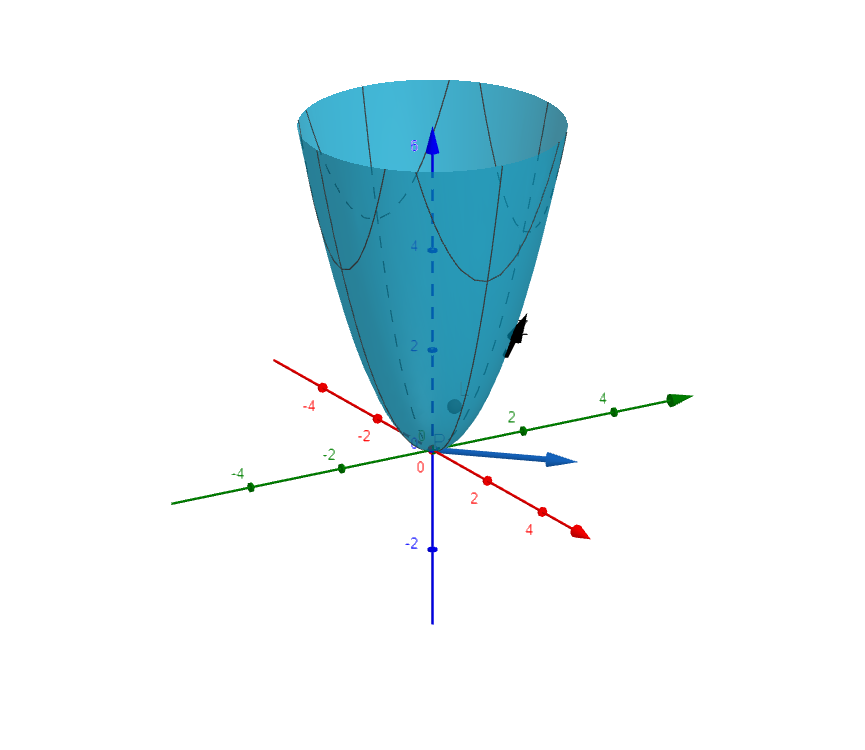
\includegraphics[width=0.6\linewidth]{../common/02_appendix/00_resources/01_gradient.png}
    \end{center}
    \caption{Gradient an der Position $(1, 1)$}
    \label{fig:01_gradient}
\end{figure}

\section{Das Gradientenabstiegsverfahren}
